\documentclass[11pt]{article}
\usepackage{lscape}
\usepackage{amsmath,amssymb}
\usepackage{amsthm}
\usepackage{float}
\usepackage{booktabs}
\usepackage{graphicx}
\usepackage{comment}
\usepackage{bm}
\usepackage{gensymb}
\allowdisplaybreaks[4]
\usepackage{geometry}
\geometry{margin=1in}
\usepackage{setspace}
\usepackage{siunitx}
\usepackage{enumitem}
\usepackage{dsfont}
\usepackage{arydshln}

\newcommand*{\vertbar}{\rule[-1ex]{0.5pt}{2.5ex}}
\newcommand*{\horzbar}{\rule[.5ex]{2.5ex}{0.5pt}}


\usepackage{graphics}
\allowdisplaybreaks

\usepackage[utf8x]{inputenc}
\usepackage{bm}

\usepackage{hyperref}
\hypersetup{
    colorlinks=true,
    citecolor = blue,
    linkcolor=blue,
    filecolor=magenta,           
    urlcolor=cyan,
}


\theoremstyle{plain}
\newtheorem{thm}{Theorem}[section]
\newtheorem{lem}{Lemma}
\newtheorem{pro}{Property}
\newtheorem{cor}{Corollary}


\theoremstyle{definition}
\newtheorem{prob}{Problem}
\newtheorem{prop}{Proposition}
\newtheorem{defn}{Definition}
\newtheorem{exmp}{Example}
\newtheorem{rmk}{Remark}
\newtheorem{con}{Conjecture}
\newtheorem{ass}{Assumption}

\usepackage{algpseudocode,algorithm}
\algnewcommand\algorithmicinput{\textbf{Input:}}
\algnewcommand\algorithmicoutput{\textbf{Output:}}
\algnewcommand\INPUT{\item[\algorithmicinput]}
\algnewcommand\OUTPUT{\item[\algorithmicoutput]}



\usepackage[labelfont=bf]{caption}

\setcounter{table}{1}
\usepackage{multirow}
\usepackage{tabularx}

\def\fixme#1#2{\textbf{[FIXME (#1): #2]}}

\def\Holder{\text{H\"{o}lder }}

\newcommand*{\KeepStyleUnderBrace}[1]{%f
  \mathop{%
    \mathchoice
    {\underbrace{\displaystyle#1}}%
    {\underbrace{\textstyle#1}}%
    {\underbrace{\scriptstyle#1}}%
    {\underbrace{\scriptscriptstyle#1}}%
  }\limits
}
\usepackage{mathtools}
\mathtoolsset{showonlyrefs=true}

\begingroup
\makeatletter
\@for\theoremstyle:=definition,remark,plain\do{%
\expandafter\g@addto@macro\csname th@\theoremstyle\endcsname{%
\addtolength\thm@preskip\parskip
}%
}
\endgroup


\usepackage{hyperref}
\hypersetup{colorlinks=true}
\usepackage[parfill]{parskip}
\usepackage{bm}
\onehalfspacing

\newcommand{\maxnorm}[1]{\left\lVert#1\right\rVert_{\infty}}
\newcommand{\Hnorm}[1]{\left\lVert#1\right\rVert_{\tH_\alpha}}
\newcommand{\nullnorm}[1]{\left\lVert#1\right\rVert}
%%%%%%%%%%%%%%%%%%%%%%%%%%%%%%%%%%%%%%%%%%%%%%%%%%%%%%%%%%%%%%%%%%%%%
%%             Math Symbols
%%%%%%%%%%%%%%%%%%%%%%%%%%%%%%%%%%%%%%%%%%%%%%%%%%%%%%%%%%%%%%%%%%%%%

%%               Bold Math
\input macros.tex
\usepackage[authoryear]{natbib}
\def\refer#1{\emph{\color{blue}#1}}
\begin{document}


\begin{center}
{\bf \Large Theory and GTEx data results}\\
Miaoyan Wang, 03/14/2021
\end{center}
\section{Convergence rate}
Consider the following constrained optimization
\begin{align}\label{eq:opt}
\min_{\tC=\{\mTheta_0, \mTheta_\ell, \bmu_\ell=(u_{l1},\ldots,u_{lK})\colon l\in[r]\}}\quad &\sum_{k\in[K]}n_k \left[\text{tr}(\mS_k\mOmega_k)-\log|\mOmega_k|\right]+\lambda\sum_{\ell\geq 1}\onenorm{\mTheta_\ell},\notag \\
\text{s.t.}\quad & \mOmega_k=\mTheta_0+\sum_{\ell\in[r]}u_{\ell k}\mTheta_\ell,\ k=1,\ldots,K,\quad \zeronorm{\mTheta_0}\leq c,\notag\\
& \bmu^T_\ell\bmu_\ell=1,\ \mathbf{1}^T\bmu_\ell=0,\ \text{supp}(\bmu_\ell)\cap \text{supp}(\bmu_{\ell'})=0,\ \text{for all }\ell\neq \ell',\ \ell,\ell'\in[r].
\end{align}

\begin{ass}\label{ass:main}We make the following assumptions on ground truth $\tC$. 
\begin{enumerate}[wide, labelwidth=!, labelindent=0pt]
\item[] 1.\ [Positiveness] There exist two positive constants $\tau_1,\tau_2>0$, such that $\tau_1\leq \phi_{\min}(\mOmega_k)\leq \phi_{\max}(\mOmega_k)\leq \tau_2$ for all $k\in[K]$, where $\phi_{\min}(\cdot)$ and $\phi_{\max}(\cdot)$ denote the minimal and maximal eigenvalues, respectively. 
\item[] 2.\ [Signal Strength]. Let $T_k\subset[p]\times[p]$ denote the set of indices of non-zero off-diagonal elements in $\mOmega_k=\entry{\omega^{(k)}_{j,j'}}$. Assume there exists a positive constant $\tau_3>0$, such that the minimal non-zero, off-diagonal entries in $\mOmega_k$ is lower bounded by $\tau_3>0$ for all $k\in[K]$; i.e., $\min_{(j,j')\in T_k, k\in[K]}\omega^{(k)}_{j,j'}\geq \tau_3$.
\item[] 3.\ [Sparseness] There exist a positive constant $c>0$ such that $\zeronorm{\mTheta_\ell}\leq c$, for all $\ell=0,1,\ldots,r$.
\item[] 4.\ [Separability] The minimal gap $\delta=\min_{\ell,\ell'}\mnormSize{}{\mTheta_\ell-\mTheta_{\ell'}}>0$. 
\end{enumerate}
\end{ass}

Notation:
\begin{itemize}
\item For simplicity, assume $n_1=\ldots=n_K=n$. 
\item Let $p$ denote the dimension of precision matrices, i.e., the number of genes.  
\item Let $s_k=|T_k|$ denote the number of non-zero off-signal elements in precision matrix $\mOmega_k$. Assume $s_1=\ldots=s_K=s$. 
\item Assume the tissue clusters are balanced in that $|\text{supp}(\bmu_1)|= \cdots =  |\text{supp}(\bmu_r)| \asymp {K\over r}$.
\end{itemize}


Note: both the following theorems assume simplified case with no intercept $\mTheta_0$. Correspondingly, we suppress the constraint $\mathbf{1}^T\bmu_\ell=0$ from algorithm~\eqref{eq:opt} and consider a slightly different version of Assumption 1:

\begin{enumerate}
\item All non-zero entries in $\{u_{\ell k}\}$ are positive and lower bounded by a constant $\delta'>0$ for all $k\in[K]$; i.e., $\min_{(\ell,k)\colon u_{\ell k}\neq 0}u_{\ell k}\geq \delta'>0$. Furthermore, there exist two positive constant $\tau_1,\tau_2>0$ such that $\tau_1\leq \phi_{\min}(\sum_{\ell\in[r]}u_{\ell k}\Theta_\ell)\leq \phi_{\min}(\sum_{\ell\in[r]}u_{\ell k}\Theta_\ell) \leq \tau_2$ for all $k\in[K]$. 
\end{enumerate}

\begin{rmk}[Intercept Effects]
The assumption of no intercept gives a slight discrepancy between current theory and algorithm. The assumption is a technical condition for a cleaner proof. I believe the case with unknown intercept can be handled with more careful bookkeeping. Will work on this. 
\end{rmk}



The following theorem provide the asymptotic convergence rate for our joint estimates in the high dimensional regime $n,p, K\to \infty$, while fixing the sparsity parameter $s$. 

\begin{thm}[Convergence of joint precision matrices estimation with growing $K$]~\label{thm:estimation}
Consider the joint Gaussian graphical model with decomposable factor constraints. Suppose Assumptions 1-3 holds. Let $\{\mS_k\colon k\in[K]\}$ be the sample covariance, $\{\hat \mTheta_1,\ldots,\hat \mTheta_r, \hat \bmu_1,\ldots,\hat \bmu_r\}$ denote the solution of~\eqref{eq:opt}, where $\lambda$ is chosen such that $\lambda\asymp {\left\{ (p+s)\log p \over Kpn\right\}}^{1/2}$. Denote $\hat \mOmega_k=\sum_{l\in[r]}\hat u_{lk}\hat \mTheta_k$ for $k=1,\ldots,K$. Then, the following accuracy bound holds with probability tending to 1,
\begin{equation}\label{eq:conclusion}
{1\over K} \sum_{k\in[K]}\FnormSize{}{\hat \mOmega_k-\mOmega_k} = \tO_p\left[{\left\{ (p+s)\log p \over Kn\right\}}^{1/2} \right].
\end{equation}
\end{thm}
\begin{rmk} Our result improves~\cite{guo2011joint} by allowing the number of tissues $K\to \infty$. In contrast to Guo et al which requires a constant $K$, our consistency results allow a more challenging case of growing $K$. Our error bound achieves consistency  as $K\to\infty$. The improvements stem from the clustering modeling of $K$ tissues into a small number of $r$ groups, where we typically have $K\gg r$.
 \end{rmk}

\begin{defn}[Misclassification rate (MCR)]
The signs of loadings $\{\bmu_\ell\colon \ell\in[r]\}$ naturally induce a clustering of $K$ tissues into $r$ groups. Specifically, let $\mU=[\mathds{1}(\bmu_1>0),\ldots,\mathds{1}(\bmu_r>0)]\in\{0,1\}^{K\times r}$ be the induced membership matrix, and $\hat \mU$ the corresponding estimate. Let $\mD=\entry{D_{ab}}\stackrel{\text{def}}{=}\mU^T\hat \mU\in\mathbb{R}^{r\times r}$ denote the confusion matrix between the two membership matrices $\mU$ and $\hat \mU$. We define the misclassification rate (MCR) as
\[
\textup{}{MCR}(\mU, \hat \mU)=\max_{b\in[r], a\neq a'\in[r]}\min \{D_{ab}, D_{a'b}\}.
\]
\end{defn}


\begin{thm}[A weak version of clustering accuracy]
Consider the same set-up as in Theorem~\ref{thm:estimation}. In addition, suppose Assumption 4 holds. Then there exist constant $c_1>0$, such that with high probability $1-n^{-c_1}$, we have
\[
\text{MCR}(\hat \mU, \mU) \lesssim {rp^2\tau_2^4\log n\over \delta^2n} \to 0, \quad \text{as }n\to\infty. 
\]
\end{thm}


\section{Data analysis}
\begin{table}[H]
\resizebox{\columnwidth}{!}{
\begin{tabular}{ccc}
Group & criteria & Tissue \\
\hline
0 &$\mu_{kl}=0$& Global \\
1& $ \mu_{k1}>0$& Spinal cord (cervical c-1), Hypothalamus,Hippocampus \\
2&$ \mu_{k1}<0$&Anterior cingulate cortex (BA24),  Frontal Cortex (BA9), Cortex\\
3&$ \mu_{k2}>0$&Putamen (basal ganglia),Nucleus accumbens (basal ganglia), Caudate (basal ganglia), \\
4&$ \mu_{k2}<0$& Cerebellum, Cerebellar Hemisphere\\
5&$ \mu_{k3}> 0$& Substantia nigra\\
6&$ \mu_{k3}<0$& Amygdala\\
\end{tabular}
}
\caption{Tissue clustering for 13 brain tissues with $p=500$ top variable genes, $r=3$, $\rho=1500$.}\label{tab:summary}
\end{table}



\begin{figure}[H]
  \centering
  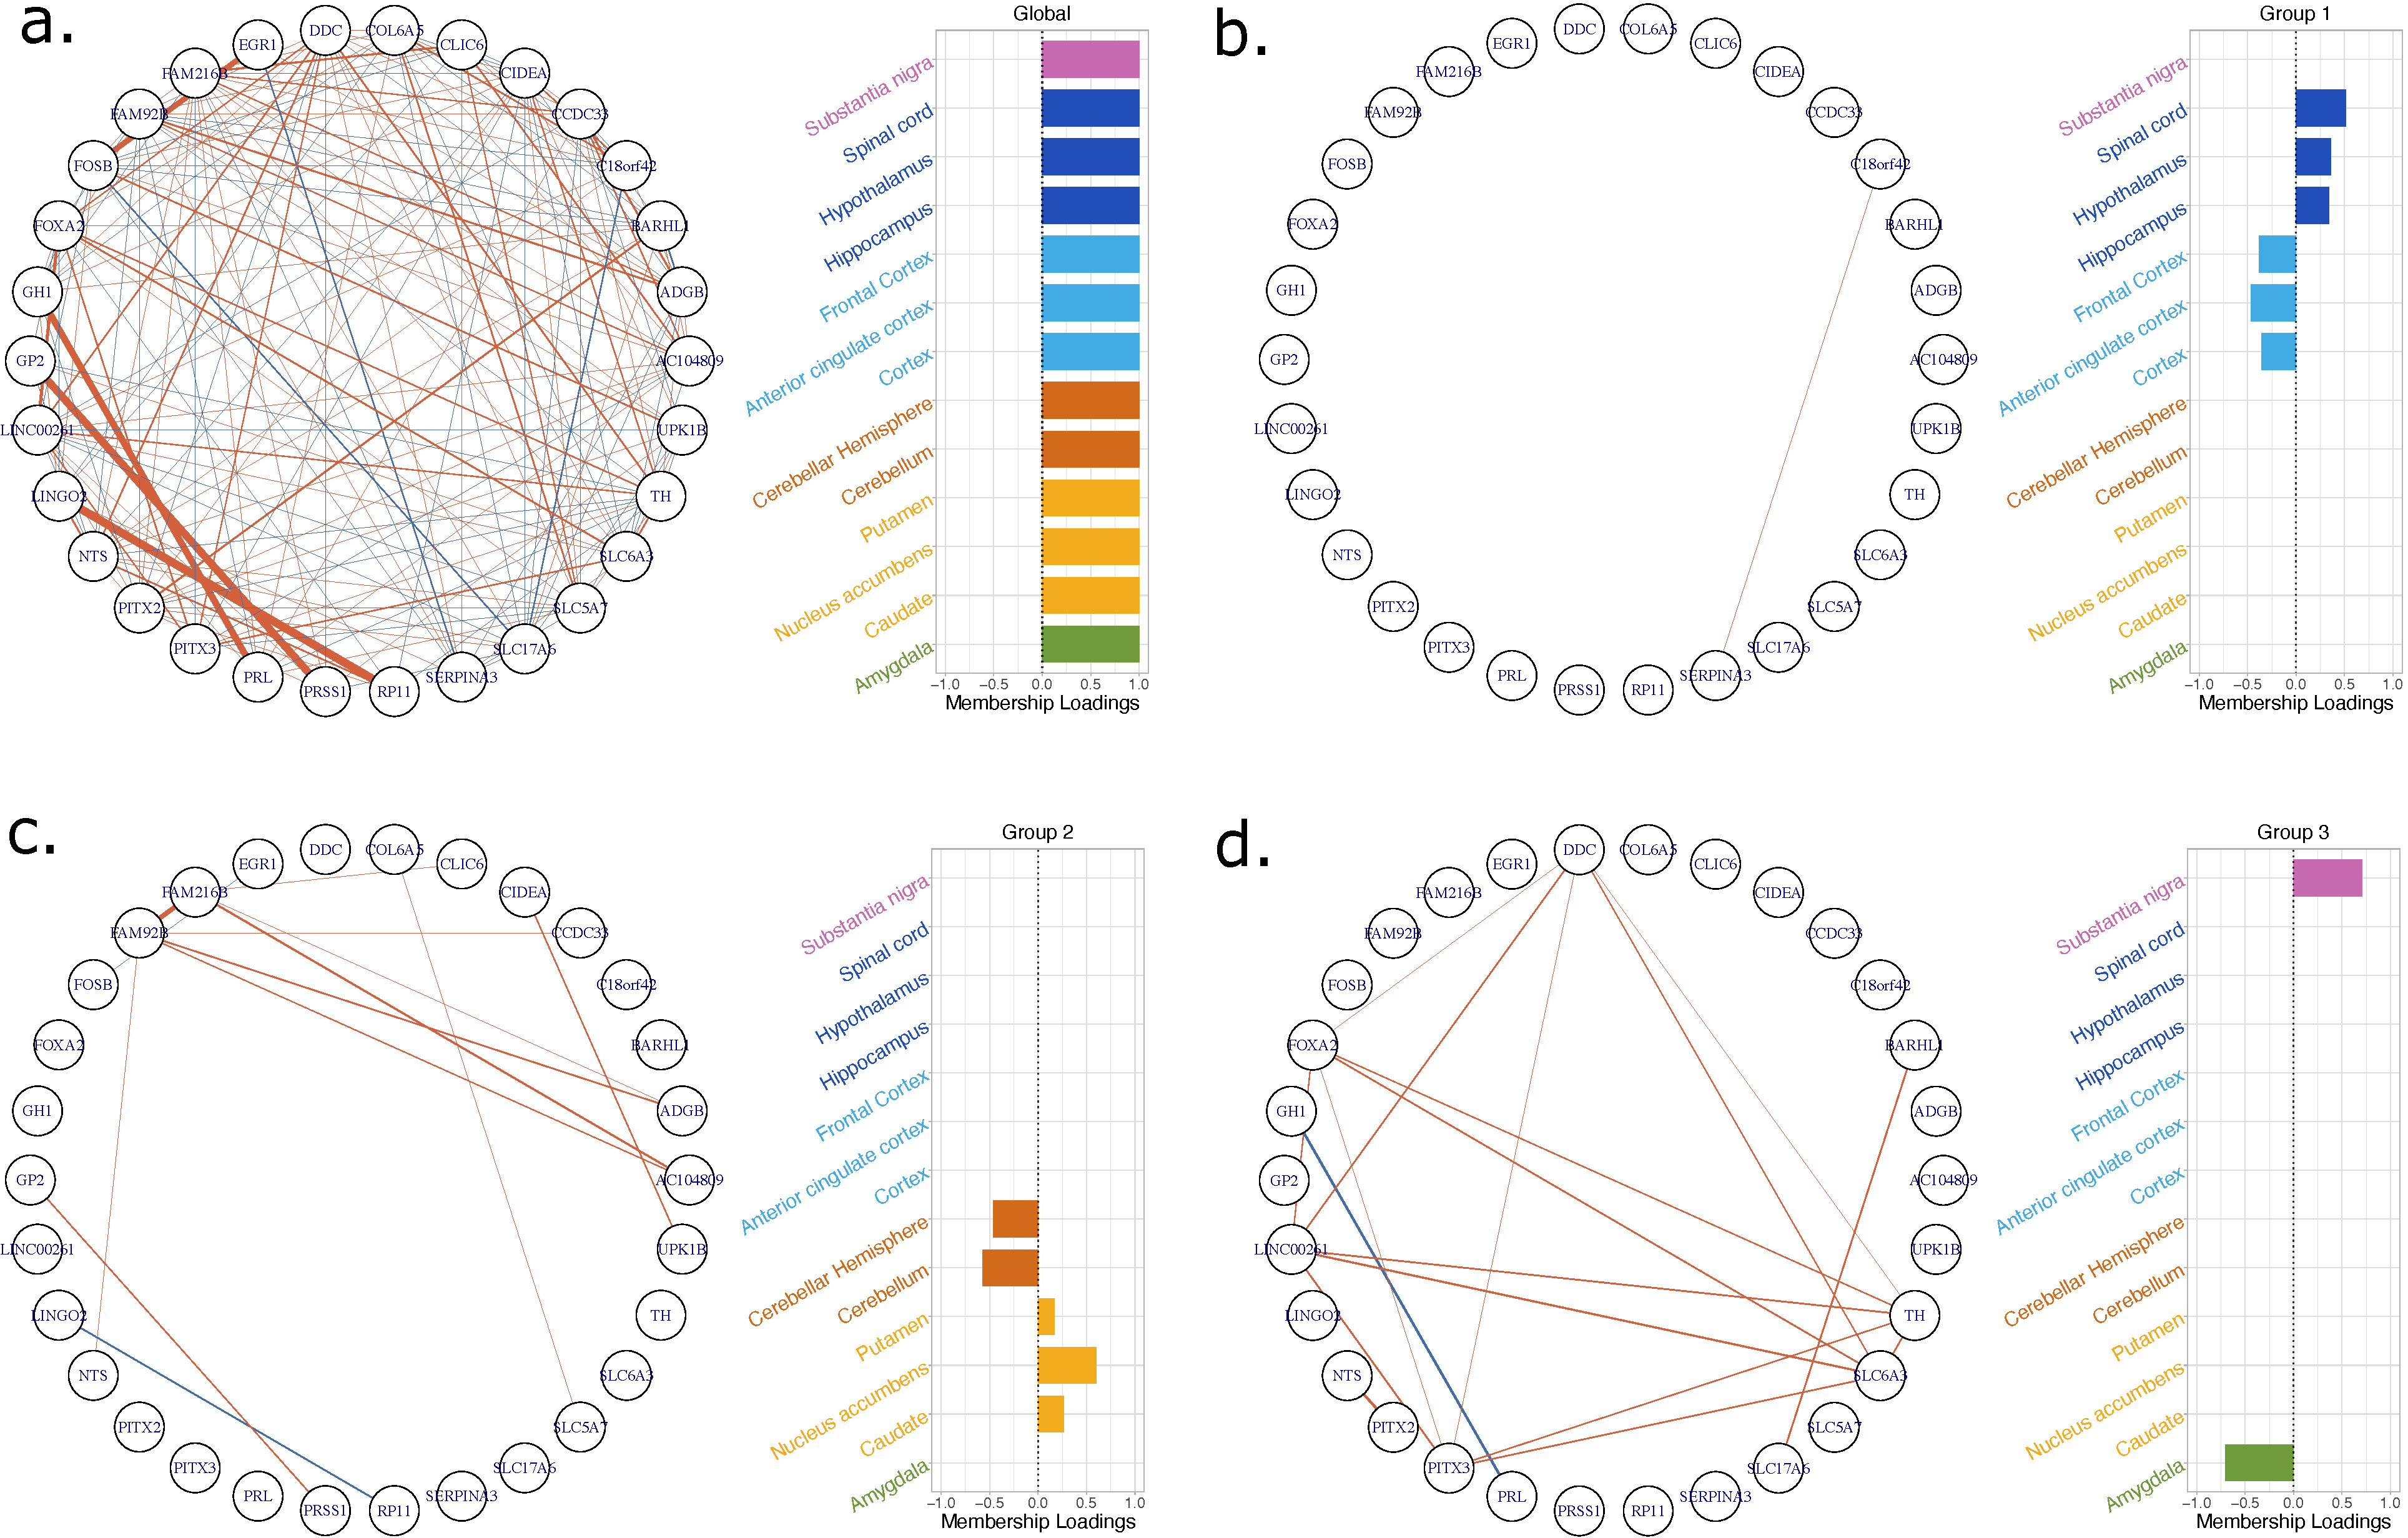
\includegraphics[width=\textwidth]{network_500}
  \caption{Tissue clusterings and differential networks based on GTEx data analysis. (a) Global network. (b) Differential network specific to cortex cluster. (c) Differential network specific to cerebellum and basal ganglia cluster. (d) Differential network specific to substantia nigra and amygdala. Blue edges represent positive entries (stronger correlation than global) whereas red edges represent negative entries (weaker correlation than global). The edge width is set proportional to the raw magnitude. For better visualization, edges with absolute value smaller than 0.05 are not shown in the global network (a). }
\end{figure}


\section{Proof}
\begin{proof}[Proof of Theorem~\ref{thm:estimation}] The accuracy for the penalized optimization with specified $\lambda$ is equivalent to the accuracy for the constrained optimization,
\begin{align}\label{eq:opt2}
\min_{\tC=\{\mTheta_0, \mTheta_\ell,\bmu_\ell\colon l\in[r]\}}\quad &\sum_{k\in[K]}n_k \left[\text{tr}(\mS_k\mOmega_k)-\log|\mOmega_k|\right],\notag \\
\text{s.t.}\quad & \mOmega_k=\mTheta_0+\sum_{\ell\in[r]}\mu_{lk}\mTheta_\ell,\ k=1,\ldots,K,\ \zeronorm{\mTheta_\ell}\leq c, \ \text{for all }\ell=0,1,\ldots,r,\notag\\
& \bmu^T_\ell\bmu_\ell=1,\ \mathbf{1}^T\bmu_\ell=0,\ \text{supp}(\bmu_\ell)\cap \text{supp}(\bmu_{\ell'})=0,\ \text{for all }\ell\neq \ell',\ \ell,\ell'\in[r].
\end{align}
Let $Q_k(\mOmega_k)=\text{tr}(\mS_k\mOmega_k)-\log|\mOmega_k|$ denote the log-likelihood for $k$-th layer. We will prove a stronger conclusion: the convergence~\eqref{eq:conclusion} holds for all estimators $\{\hat \mOmega_k\}$ that satisfy 
\begin{enumerate}
\item P1. $\sum_{k\in[K]}n_kQ_k(\hat \mOmega_k)\leq \sum_{k\in[K]}n_kQ_k(\mOmega_{k,\text{true}})$. 
\item P2. $\{\hat \mOmega_k\}$ satisfy the constraints specified in~\eqref{eq:opt2}. 
\end{enumerate}
Let $\Delta_k=\hat \mOmega_k-\mOmega_k$. Define the Taylor expansion around ground truth $\{\mOmega_k\}$, 
\[
F(\Delta_1,\ldots,\Delta_K)=\sum_{k\in[K]}\left\{\text{tr}(\mS_k(\mOmega_k+\Delta_k))-\text{tr}(\mOmega_k)-\log|\mOmega_k+\Delta_k|+\log|\mOmega_k|\right\}=:I_1+I_2,
\]
where 
\begin{align}
I_1&=\sum_{k\in[K]}\text{tr}((\mS_k-\mSigma_k)\Delta_k),\notag\\
I_2&=\sum_{k\in[K]}(\tilde \Delta_k)^T\int_{0}^1(1-v)(\mOmega_k+v\Delta_k)^{-1}\otimes(\mOmega_k+v\Delta_k)^{-1}dv\tilde \Delta_k, \ \text{with }\tilde \Delta_k  \in [0,\Delta_k].
\end{align}
By definition, every estimate satisfying P1 must have $F(\Delta_1,\ldots,\Delta_K)\leq 0$. 
With similar calculations as Guo et al (details omitted), we have
\begin{align}\label{eq:1}
I_1&\leq C\left( {\log p \over n}\right)^{1/2} \sum_{k\in[K]}\left( |\Delta^{\text{off}}_{T_k}|_1+|\Delta^{\text{off}}_{T^c_k}|_1\right) + C_2\left({p\log p\over n} \right)^{1/2}\sum_{k\in[K]}\FnormSize{}{\Delta^{\text{diag}}_k},\notag\\
 I_2&\geq {1\over 4\tau^2_2}\sum_{k\in[K]}\FnormSize{}{\Delta_k}^2,
\end{align}
where $\Delta^{\text{off}}_{T_k}$ denotes the off-signal entries of $\Delta$ restricted to set $T_k$ (correct non-zero edges), $\Delta^{\text{off}}_{T^c_k}$ denotes the off-diagonal entries of $\Delta$ restricted to $T^c_k$ (false non-zero edges), and $\Delta^{\text{diag}}_k$ denotes the diagonal entries.  
Note that $|\Delta^{\text{off}}_{T_k}|_1 \leq \sqrt{s}\FnormSize{}{\Delta_k}$, so we only need to control $|\Delta_{T^c_k}|_1$. Expanding the expression, we have
\begin{equation}\label{eq:2}
|\Delta_{T^c_k}|_1=|\hat \Theta_{0,T^c_k}+\hat \mu_{1k}\hat \Theta_{1,T^c_1}+\ldots+\hat \mu_{rk}\Theta_{k,T^c_k}|_1\leq (r+1)c\FnormSize{}{\Delta_k}, 
\end{equation}
for all $k\in[K]$. Now we consider estimate that satisfy $F(\Delta_1,\ldots,\Delta_K)\leq 0$, i.e.
\begin{equation}\label{eq:3}
I_2\leq -I_1\leq|I_1|.
\end{equation}
Plugging~\eqref{eq:1}-\eqref{eq:2} into~\eqref{eq:3} gives
\[
{1\over 4\tau^2_2}\sum_k\FnormSize{}{\Delta_k}^2\leq (C_1+C_2)\left( {(p+q)\log p\over n}\right)^{1/2}\sum_k\FnormSize{}{\Delta_k}.
\]
Using the fact that $\sum_k\FnormSize{}{\mA_k}^2\geq {1\over K} \left( \sum_k\FnormSize{}{\mA_k} \right)^2$, we have
\[
\sum_{k\in[K]}\FnormSize{}{\Delta_k}=\sum_{k\in[K]}\FnormSize{}{\hat \mOmega_k-\mOmega_k} = \tO_p\left[{\left\{ (p+s)\log p \over n\right\}}^{1/2} \right].
\]
\end{proof}

\bibliographystyle{plain} % Style BST file (imsart-number.bst or imsart-nameyear.bst)
\bibliography{tensor_wang}    

\end{document}
